\documentclass[14pt, a4paper, oneside, bold]{extarticle}

\usepackage[english, russian]{babel}
\usepackage[utf8]{inputenc}
\usepackage{amsmath}
\usepackage{amssymb}
\usepackage{graphicx}
\usepackage{multicol}
\usepackage[14pt]{extsizes}
\usepackage{listingsutf8}
\usepackage{color}
\usepackage{wrapfig}
\usepackage{enumerate}
\usepackage{amsthm}
\usepackage{indentfirst}
\usepackage{tabularx}

\usepackage{setspace}
\singlespacing
\onehalfspacing
\doublespacing

\allowdisplaybreaks
\binoppenalty = 10000
\relpenalty = 10000
\textheight = 23cm
\textwidth = 20cm
\oddsidemargin = 0pt
%\topmargin = -1.5cm
\parskip = 0pt
\tolerance = 2000
\flushbottom

\usepackage[left=30mm, right=20mm, top=20mm, bottom=30mm, nohead, footskip=10mm]{geometry}
% bottom=2cm, bindingoffset=0cm]

\pagestyle{plain}

\renewcommand{\thesection}{\arabic{section}}

\begin{document}

\allowdisplaybreaks[1]

\begin{titlepage}
\setstretch{1}
\begin{center}
\ \vspace{-1.5cm}

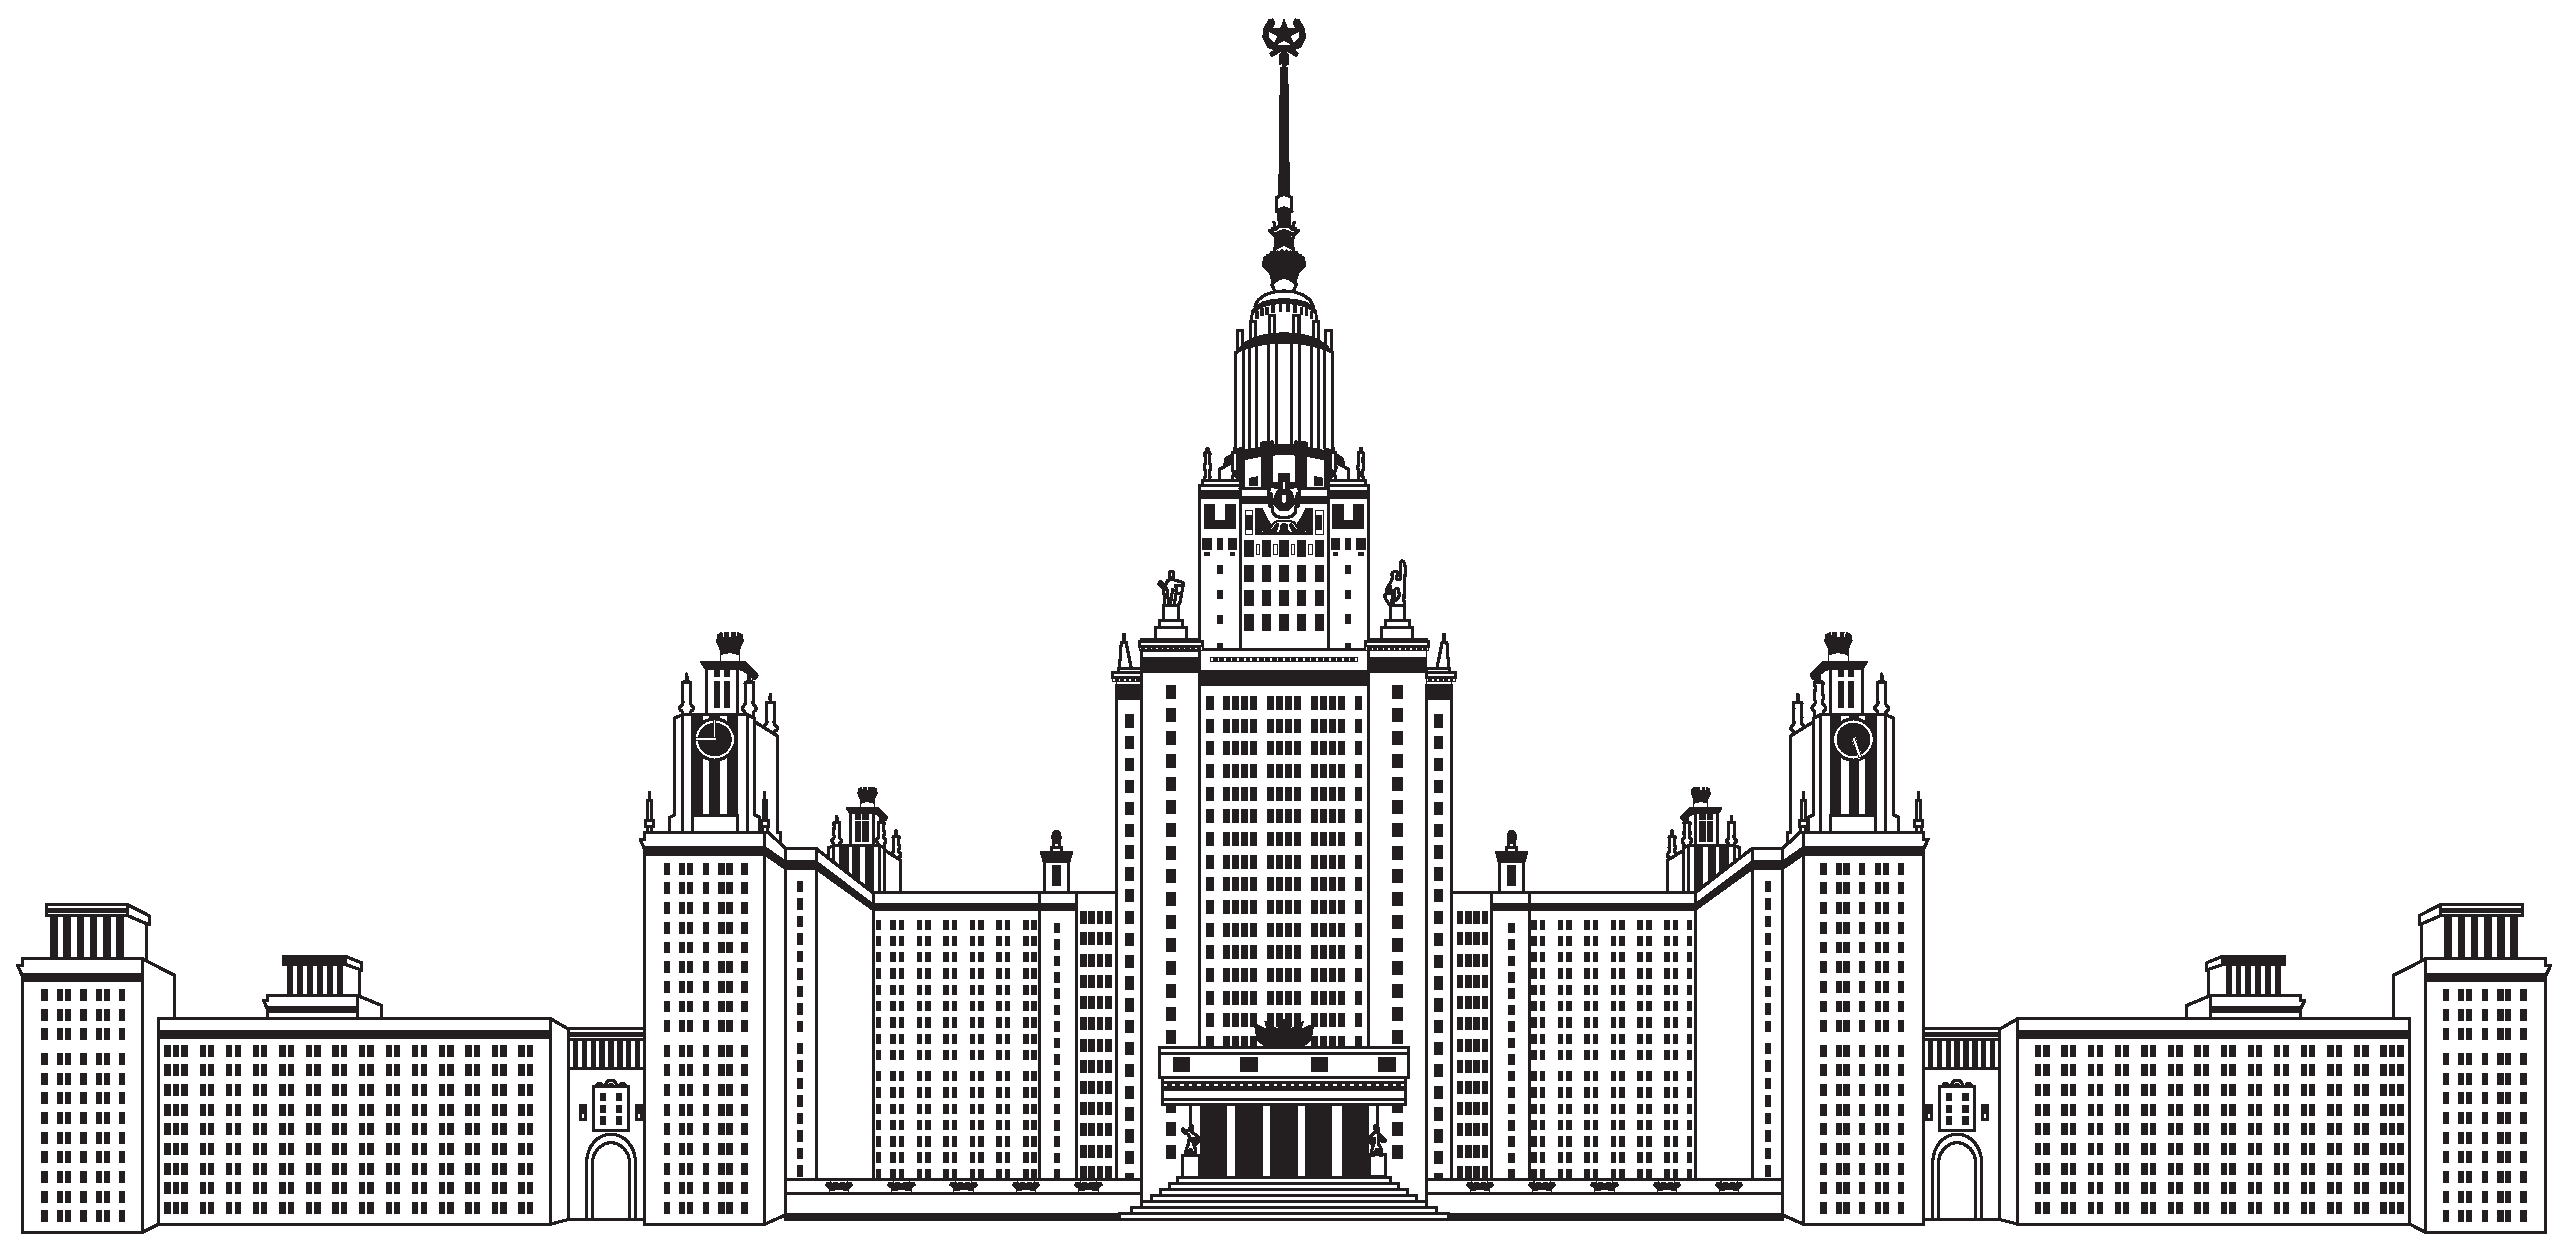
\includegraphics[width=0.5\textwidth]{data/images/msu_logo.eps}\\
{\bfseries Московский государственный университет имени М.В. Ломоносова \\
Факультет вычислительной математики и кибернетики\\
Кафедра исследования операций}

\vspace{3cm}

{\Large Лаврухин Ефим Валерьевич}

\vspace{1cm}

{\Large\bfseries
Применение нейронных сетей для решения задачи оптимальной сегментации томографических
изображений геологических пород\\}

\vspace{1cm}

{\textbf \large МАГИСТЕРСКАЯ ДИССЕРТАЦИЯ}
\end{center}

\vfill

\begin{flushright}
  \textbf{Научный руководитель:}\\
  к.ф.-м.н., доцент\\
  Д.В.~Денисов
\end{flushright}

\vfill

\begin{center}
Москва, 2018
\end{center}

\vspace{1cm}

\enlargethispage{2\baselineskip}

\end{titlepage}

\setstretch{1.5}

\newpage

\tableofcontents

\newpage


\section{Введение} \label{intro}

В настоящее время добыча полезных ископаемых требует большое количество 
данных о разрабатываемых породах-коллекторах. Эти данные получают в том числе с помощью методов цифровой петрофизики, которые работают с  
2-D или 3-D изображениями, сделанными с помощью рентгеновской томографии \cite{1}. Большинство изображений строения пород представлены в градациях серого, которые указывают на интенсивность поглощения рентгеновских лучей. На практике любой метод численного расчета характеристик исходных пород состоит из нескольких отдельных этапов. 
И первый этап -- это сегментация входного изображения, разделение его
на несколько различных фаз по плотности вещества. В простейшем случае выполняется бинаризация -- разделение на твёрдую породу и поры \cite{2}. 

Цель данной работы -- применить методы глубинного обучения, а именно полносвёрточные нейронные сети, для задачи сегментации изображений геологических пород.

Существует большое количество методов сегментации. Они существенно отличаются в принимаемых предположениях о входных изображениях и используемом математическом аппарате. Вот некоторые из них: градиентные \cite{13}, морфологические \cite{17}, случайные поля \cite{14}, методы Монте-Карло \cite{16}. У этих методов есть ряд достоинств: присутствует математическая формализация, относительная простота постановки задачи, интерпретируемость результатов. Но в то же время все они обладают серьёзным недостатком -- в них присутствуют гиперпараметры, которые сильно влияют на качество результата. Это делает затруднительным их применение без оператора, который контролирует процесс и подбирает нужные значения параметров для  конкретных входных данных. 

Относительно недавно появились методы сегментации с использованием машинного обучения. Классические методы машинного обучения уже применялись в сегментации изображений геологических пород \cite{3}, \cite{4}, \cite{5}.

Сейчас свёрточные нейронные сети являются, фактически, state-of-the-art в задачах обрабоки изображений и используются во многих прикладных областях: биологии \cite{6}, медицине \cite{18}, распознавании образов \cite{11}. На текущий момент выпущено достаточно много работ, в которых исследуются методы глубинного обучения для решения связанных с сегментацией пород задач. В частности для  построения стохастической реконструции пород с последующим моделированием физических свойств \cite{7}, \cite{8}, \cite{9}, \cite{10}. Но статей, в которых глубинное обучение применяется для сегментации геологических пород, крайне мало. 

В ходе работы для достижения поставленной цели решались следующие 
задачи:
\begin{enumerate}
	\item Постановка задачи оптимальной сегментации как задачи нелинейной оптимизации(разделы \ref{seg_def}, \ref{seg_features}, \ref{seg_supervised}).
	
	\item Выбор полносвёртночной архитектуры нейронной сети, 
которая выполняет сегментацию изображений томограмм(раздел \ref{seg_nn}).

	\item Построение стабильного алгоритма обучения сети(раздел \ref{seg_optimization}).
	
	\item Решение проблемы отсутствия размеченных обучающих данных(раздел \ref{seg_tasks}).
	
	\item Проверка модели на реальных данных(раздел \ref{seg_results}).
	
\end{enumerate}
  
\newpage


\section{Постановка задачи сегментации} \label{seg_def}

Сначала рассмотрим простейшую постановку задачи сегментации изображения.

\begin{problem}[framed]{Задача сегментации}
  Task: & Define a new ``problem'' environment. \\
  Problem: & The only keywords you can use to search on Google
    are ``latex'' ``problem'' ``definition'' ``environment''. \\
  Solution: & Be patient.
\end{problem}

Дано исходное изображение 
	$S = (s_{ij})_{i=1, j=1}^{H, W},\ s_{ij} \in [0, 1]$, где 
$H$ -- высота изображения, $W$ -- ширина изображения. 
Требуется для каждого пикселя найти соответствующий ему сегмент изображения, 
т.е. найти соответствие $s_{ij} \rightarrow m_{ij},\ m_{ij} \in C = \{ 0, ... , N_c-1 \} $,
где $N_c$ -- число различных сегментов.

Подразумевается, что для каждого изображения $S$ существует 
истинное(возможно, не одно) сегментированное изображение $M$.
Поэтому можно перейти к следующей постановке задачи: найти алгоритм сегментации $\mathcal{A}$, такой, что он преобразует любое 
изображение $S$ в  маску $\hat{M}$:
\begin{equation}
	\mathcal{A}(S | \theta) = \hat{M}
\end{equation} 
, где $\theta$ -- настраеваемые параметры нашего алгоритма.

Возникают следующие вопросы:
\begin{enumerate}
	\item Как выбрать алгоритм $\mathcal{A}$?
	\item Как настроить параметры $\theta$?
	\item Как оценить ошибку алгоритма?
\end{enumerate}
Существуют различные способы рещения этих вопросов.
Выбор алгоритма $\mathcal{A}$ и способа оценки качества его работы обуславливается задачей и необходимыми результатами. 
Подбор параметров $\theta$ выполняется непосредственно 
оператором, с помощью 
обучения без учителя(unsupervised learning) или с помощью обучения с учителем(supervised learning).

\newpage


\section{Особенности задачи сегментации геологических пород} \label{seg_features}

Для задачи сегментации томографических изображений геологических пород существуют некоторые особенности. 
 
Дан исходный стек изображений 
	$S = (s_{ijk})_{i=1, j=1, k=1}^{H, W, D},\ s_{ijk} \in [0, 1]$, где 
$H$ -- высота изображения, $W$ -- ширина изображения, $D$ -- количество изображений. 
Требуется для каждого пикселя найти соответствующую ему метку класса, 
т.е. найти соответствие $s_{ijk} \rightarrow m_{ijk},\ m_{ijk} \in C = \{ 0, 1 \} $, где класс $0$ соответствует порам, класс $1$ -- твердому веществу.

Особенности данной задачи:
\begin{enumerate}
	\item Работа с 3-D изображениями.
	\item Двухклассовая сегментация.
	\item Наличие сегментированных стеков, для которых изместно 
	$\hat{M}$ некоторого ''качественного'' алгоритма.	
\end{enumerate}

Как правило, данная задача на практике решалась методами MRF, snakes и некоторыми другими. Собрана некоторая база изображений 
$S, \hat{M}$, качество сегментации которых оценивалось оператором.

В таком случае естественно перейти к задаче обучения с учителем(supervised learning), чтобы использовать накопившуюся библиотеку сегментированных изображений. 

\newpage


\section{Постановка задачи supervised сегментации} \label{seg_supervised}


Дано пространство объектов $X$ и пространтсво ответов $Y$. Между ними существует соответствие(функция) $f: X \rightarrow Y$. 

Требуется наилучшим образом приблизить соответствие $f$ при помощи 
параметрического семества функций $f_{\theta}$ и множеством примеров отображения $f: \{(X_1,\ Y_1),\ ... ,\ (X_N,\ Y_N) \}
	,\ f(X_i) = Y_i ,\ i = \overline{1, N}$.

В конкретном случае множество примеров из пространства $X$ задаётся в виде:
\begin{equation}
	\hat{X} = \{ X_1, ..., X_N \},\ X_k = (x_{ij})_{i=1, j=1}^{H, W}
                       	   ,\ x_{ij} \in [0, 1]
\end{equation}
и множество ответов из $Y$ задаётся в виде:
\begin{equation}
	\hat{Y} = \{ Y_1, ... , Y_N \},\ Y_k = (y_{ij})_{i=1, j=1}^{H, W}
							,\ y_{ij} \in \{ 0, 1 \}.
\end{equation} 

Конкретное значение параметра $\theta$ параметрического семейства $f_{\theta}$ выбирается изходя из функционала качества модели(функции эмпирического риска):
\begin{equation}\label{opt}
	Q \bigl( \theta, (\hat{X}, \hat{Y}) \bigr) = 
		\sum \limits_{i=1}^{N} \mathcal{L} 
		\bigl( f_{\theta}(X_i), Y_i \bigr)
		\longrightarrow \min \limits_{\theta}.
\end{equation}

Задача состоит в выборе параметрического семейства $f_\theta$, 
функции потерь $\mathcal{L}(\overline{Y}, Y)$ и решении 
оптимизационной задачи (\ref{opt}).

\newpage


\section{Архитектура нейронной сети} \label{seg_nn}

В качестве семейства функций $f_{\theta}$ в работе использовалась 
полносвёрточная нейронная сеть (fully-connected convolutional neutral network). В качестве основы была выбрана архитектура U-net, которая зарекомендовала себя в решении задач биологии(выделение границ клеток). 

В архитектуру были внесены незначительные изменения: уменьшено количество свёрточных фильтров, добавлен padding, изменена функция активации на ELU.

Сеть представляет из себя композицию линейных
(свертки (\ref{conv}), конкатенация (\ref{concat}), и transposed convolutions, действие которых эквивалентно обратному действию свёрточных слоев, т.е по выходу свёрточного слоя $y$ и фильтрам $w$ получается вход свёрточного слоя $x$) 
и нелинейных преобразований
(активации (\ref{ELU}), (\ref{softmax}), pooling (\ref{pooling})) которые применяются последовательно. 
Вероятности на выходе обеспечиваются с помощью 
softmax-преобразования выхода сети: 

\begin{equation} \label{ELU}
	y = \begin{cases} 
		& x ,\ \text{при $x \geq 0$}, \\	
		& e^x - 1 ,\ \text{при $x < 0$}.
	\end{cases}
\end{equation}

\begin{equation} \label{softmax}
\begin{aligned}
	& y_{c, i, j} = \frac{ e^{x_{c, i, j}} }
		{ \sum \limits_{l=1}^{C} e^{x_{l, i, j}} } \\
	& x \in \mathbb{R}^{C \times W \times H}
		,\ y \in \mathbb{R}^{C \times W \times H}
\end{aligned}
\end{equation}

\begin{equation} \label{conv}
\begin{aligned}
	y_{c, i, j} & = \sum \limits_{l=1}^{C} 
		\sum \limits_{m=1}^{min(W - i, K)}
		\sum \limits_{n=1}^{min(H - j, K)} 
		x_{l, i + m, j + n} \ w^c_{l, m, n} \\
	& ,\ c = \overline{1, T} 
		,\ i = \overline{1, W}
		,\ j = \overline{1, H} \\
	& \text{, где $x \in \mathbb{R}^{C \times W \times H}$
		- вход свёртки} \\
	& \text{, $y \in \mathbb{R}^{T \times W \times H}$ 
		- выход свёртки} \\
	& \text{, $w^c \in \mathbb{R}^{C \times K \times K}$
		- фильтры свёрток} \\
	& \text{, $c=\overline{1, C}$ - количество свёрток}.
\end{aligned}
\end{equation}

\begin{equation} \label{concat}
\begin{aligned}
	& z_{c, i, j} = \begin{cases}
		& x_{c, i, j} \text{, если $c \leq C$,} \\
		& y_{c - C, i, j} \text{, если $c > C$}
	\end{cases} \\
	& \text{, где $x \in \mathbb{R}^{C \times W \times H}$
	,\ $y \in \mathbb{R}^{T \times W \times H}$ 
	,\ $z \in \mathbb{R}^{(T + C) \times W \times H}$}
\end{aligned}
\end{equation}

\begin{equation} \label{pooling}
\begin{aligned}
	y_{c, i, j} & = \max \limits_{
		\substack{
			m=\overline{1, min(W - i, K)}
			\\ n=\overline{1, min(H - j, K)}}}
		x_{c, i K + m, j K + n} \\
	& \text{, где $x \in \mathbb{R}^{C \times W \times H}$ 
		- вход pooling'а} \\
	& \text{, $y \in \mathbb{R}
		^{C 
		  \times \bigl[ \frac{W + K - 1}{K} \bigr] 
		  \times \bigl[ \frac{H + K - 1}{K} \bigr] }$ 
		- выход pooling'а} \\
	& \text{, $K$ - размер ядра pooling'а}.
\end{aligned}
\end{equation}

Модель реализует следующее отображение: 
\begin{equation} \label{model}
\begin{aligned}
	& f_{\theta}(x) = y, \\
	& x \in \mathbb{R}^{1 \times H \times W}
		,\ y \in 
		\mathbb{R}^{2 \times H \times W}
\end{aligned}
\end{equation}
, где первая первая размерность - число каналов изображения(на входе один, потому что изображение grayscale; на выходе два: в первом канале вероятность того, что текущий пиксель - это пора, во втором - что это твёрдое вещество), последние две размерности - это размер изображений. В качестве оптимизируемых параметров модели $\theta$ выступает совокупность весов convolutional и transposed convolutional слоёв.

\newpage


\section{Оптимизация модели} \label{seg_optimization}

\subsection{Оптимизируемый функционал}

Для финальной постановки задачи осталось выбрать функцию потерь 
$\mathcal{L}(\overline{Y}, Y)$. Поскольку выход модели (\ref{model})
является бинарными вероятностями, подходящей функцией является кросс-энтропия:
\begin{equation} \label{cross-entropy}
	CE(\overline{Y}, Y) = \sum \limits_{i=1, j=1}^{W, H} \Bigl(
		Y_{ij} \log \overline{Y}_{0ij} 
		+ (1 - Y_{ij}) \log (1 - \overline{Y}_{1ij}) \Bigr).
\end{equation}

Выбор обуславливается тем, что функция гладкая, выпуклая, минимум достигается 
при выборе с помощью прогноза $\overline{Y}$ верного класса и функция 
имеет адекватную вероятностную интерпретацию.

Так же в качестве метрики качества в задачах сегментации используют коэффициент Жаккара: 
\begin{equation} \label{jaccard}
	J(A, B) = \frac{|A \cap B|}{|A \cup B|} 
\end{equation}
, где в качестве множеств $A$ и $B$ выступают множество пикселей, отнесённые к 
первому(второму) классу моделью, и множество пикселей, образующих правильный ответ для первого(второго) класса.

Коэффициент Жакарра (\ref{jaccard}) нельзя использовать для обучения модели напрямую, потому что для его вычисления требуется определённый(метка конкретного класса) прогноз модели, а модель 
(\ref{model}) возвращает вероятности меток. При переходе от вероятности к меткам по порогу(например, при $p<0.5$ предсказывается первый класс, иначе - второй) функция перестаёт быть гладкой. Поэтому в качестве функции потерь можно использовать гладкую аппроксимацию (\ref{jaccard}). Можно придумать различные виды аппроксимации, в данной работе применялась следующая:
\begin{equation} \label{smoothed_iou}
	sIOU(\overline{Y}, Y) = \sum \limits_{i=1, j=1}^{W, H}
		\frac{Y_{ij} \overline{Y}_{ij} + \varepsilon}
		{Y_{ij} + \overline{Y}_{ij} 
			- Y_{ij} \overline{Y}_{ij} + \varepsilon}.
\end{equation} 
 
Можно убедиться, что при ''стремлении'' 
$\overline{Y}$ к $Y$ значение $sIOU(\overline{Y}, Y)$ стремится к $J(A(\overline{Y}, \tau), Y)$ при любом выборе порога $\tau$. В выражении (\ref{smoothed_iou}) фигурирует 
константа $\varepsilon$(на практике, например, $\varepsilon=10^{-5}$), которая используется для вычислительной стабильности.
 
Итоговая фунция потерь, которая использовалась для оптимизации модели, имеет вид:
\begin{equation} \label{final_loss}
	\mathcal{L}(\overline{Y}, Y) = CE(\overline{Y}, Y)
		+ \gamma \log \bigl( sIOU(\overline{Y}, Y) \bigr)
\end{equation}
, где $\gamma$ - коэффициент соотношения функций потерь. Величина (\ref{smoothed_iou}) находится под логарифмом для коррекции соотношения к величине (\ref{cross-entropy}).

\subsection{Метод оптимизации}

Последним шагом для завершения модели является выбор метода решения 
задачи (\ref{model}) для функции потерь (\ref{final_loss}).

Для задач оптимизации параметров нейронных сетей характерны следующие особенности:
\begin{itemize}
	\item Огромное число оптимизируемых параметров
	
	\item Непрерывное пространство оптимизируемых параметров
	
	\item Возможность аналитического вычисления градиентов с помощью
back propogation
		
	\item Сложная структура оптимизируемого функционала: отсутствие 	выпуклости, множество седловых точек и локальных минимумов
	
	\item Большой размер обучающей выборки  
\end{itemize} 
	
В связи с непрерывной структурой пространства параметров и возможностью вычислять аналитические градиенты эвристические(отжиг, генетические алгоритмы) методы для оптимизации параметров нейронных сетей применяются редко. Из-за огромного числа параметров квадратиные методы оптимизации не применимы, даже квазиньютовоские методы, как правило, оказываются неоправданно медленными. Для обучения используются тренировочные выборки большого размера, поэтому методы оптимизации должны обрабатывать выборку по батчам. 

По этим причинам задачи оптимизации в нейронных сетях решаются в основном с помощью вариаций стохастического градиента. В основном используются варианты с моментумом(для выхода из седловых точек и плохих локальных минимумов) и адаптивным темпом обучения. В данной работе в качестве метода оптимизации использовался ADAM.

\newpage


\section{Ход работы} \label{seg_tasks}

\subsection{Прикладная задача}

Задача, которая стояла перед началом работы, - проверить возможность применения глубинного обучения для сегментации изображений геологических пород. В настоящее время для решения данной задачи используются методы без обучения, поэтому для настройки параметров методов необходим оператор, который будет валидировать полученные результаты.
Методы глубинного обучения выглядят привлекательными для данной задачи по следующим причинам:
\begin{itemize}
	\item Автоматическая оптимизации параметров, а значит полной 	независимости от оператора
	
	\item Оптимизация на этапе обучения, отсутствие оптимизации на этапе прогноза 
	
	\item Высокая обобщающая способность, возможность построения универсальной модели для широкого класса пород
	
\end{itemize}
 
\subsection{Данные для моделирования}

Из-за наличия обучения возникает проблема формирования обучающей выборки: сейчас не существует коллекции правильно размеченных томограмм геологических пород. Альтернативой является использование в качестве обучающей выборки изображений, полученных с помощью других методов под контролем оператора. Именно такой путь я выбрал в данной работе.

В качестве тренировочной выборки были выбраны образцы следующих пород: карбонаты(4 образца, названия: carb96558, carb71, carbRNF, SPE\_carb)  песчаники(4 образца, названия: SoilAh-1, SoilB-1, SoilB-2, TiTree\_1, TiTree\_2) и почвы(3 образца, названия: Urna\_22, Urna\_30, Urna\_34). В	качестве истинной сегментации использовались изображения, полученные с помощью метода CAC(convergene active contours).


\subsection{Постановка эксперимента}

В ходе работы было построено 7 молелей, каждая модель обучалась на 700 парах изображение-сегментация, изображения размера $700\times700$: 
\begin{itemize}
	\item Модель для карбонатов обучалась на образце carb96558
	
	\item Модель для почв обучалась на образце SoilB-2
	
	\item Модель для песчаников обучалась на образце Urna\_22
	
	\item Парная модель для карбонатов и почв обучалась на образцах carb96558 и SoilB-2, обучающие пары распрелелялись в пропорции $1:1$
	
	\item Парная модель для карбонатов и песчаников обучалась на образцах carb96558 и Urna\_22, обучающие пары распрелелялись в пропорции $1:1$
	
	\item  Парная модель для песчаников и почв обучалась на образцах Urna\_22 и SoilB-2, обучающие пары распрелелялись в пропорции $1:1:1$
\end{itemize}

В качестве образцов для обучения намерено выбирались наименее ''особенные'' образцы, чтобы проверить обобщающую способность модели, возможности справляться с объектами с отличниями от обучающей выборки.

\newpage


\section{Результаты} \label{seg_results}

\subsection{Обучение моделей}

Процесс обучения состоял из 10 эпох. В каждой эпохе модель обучалась на случайной подвыборке тренировочной выборки, размер случайной подвыборки $\frac{1}{5}$ от всей выборки. Таким образом каждый обучающий пример подавался в модель в среднем 2 раза за время обучения. В качестве входных данных модели подавались 2-D фрагменты изображений образцов размером $64 \times 64$, которые были получены разделением исходных изображений на части с минимальным наложением.
Все изображения образца расположены в одной плоскости, 3-D структура образца формируется путём ''наложения'' изображений друг на друга.

В качестве целевого функционала использовался (\ref{final_loss}) с 
$\gamma=1, \varepsilon=10^{-5}$. Модель обучалась с помощью метода 
ADAM с параметрами \\
$\alpha=10^{-3}, \beta_1=0.9, \beta_2=0.999$. Так же использовалось 
мультипликативное понижение темпа обучение, т.е. на каждой эпохе 
$\alpha$ домножалось на темп снижения $\lambda=\sqrt[10]{10^{-2}}$( такая константа выбрана для того, чтобы на последней эпохе темп обучения снизился до $\alpha=10^{-5}$).

В процессе обучения отслеживалась величина оптимизируемого функционада (\ref{final_loss}), а так же следующие функции качества:
logistic loss (\ref{cross-entropy}), sIOU (\ref{smoothed_iou}) и 
точность предсказаний по фиксированному порогу $\tau=0.5$. 

На () приведены примеры кривой обучения для нескольких моделей. Видно, что метрики ведут себя согласованно(т.е. сохраняется тренд повышения качества по всем метрикам). К последним эпохам метрики выходят на плато, что говорит о стабилизации параметров модели.


\subsection{Выбор порога вероятности} 

В рамках прикладной задачи по обработке образцов томограмм геологических пород от модели требуется получение бинарной маски предсказанных классов для пикселей исходного изображения. Модель 
(\ref{model}) предоставляет распределение вероятностей классов. Для того, чтобы перейти от вероятностей к бинарным меткам, треуется выбрать порог перехода $\tau$(для отслеживания прогресса в обучении модели, как указано в предыдущем порразделе, выбиралось $\tau=0.5$).
Поскольку конечная цель данной работы - это получение модели с высокой обобщающей способностью, применимой к различным видам пород, подбор параметра порога $\tau$ выглядит затруднительной задачей(в самом деле, он может быть разным для разных образцов пород, а значит его нельзя заранее получить для образцов, которые обрабатываются впервые, и для которого нет аналогичных обработанных образцов).

В ходе экспериментов было установлено, что 
модель (\ref{model}), которая тренируется для минимизации функции качества (\ref{final_loss}), имеет необычную(нехарактерную для подобных моделей) плотность распределения вероятностей пикселей $f(p)$ - вся вероятностая масса расположена вблизи 0 и 1. Это значит, что качество бинарного прогноза модели устойчиво к выбору порога в широком интервале(в эксперимента любой порог $\tau \in [0.1,\ 0.9]$ показывал примерно аналогичный результат). Из вышесказанного следует, что данное свойство модели имеет большое практическое значение. 

\subsection{Оценка ошибок в разных плоскостях}

Поскольку обучающие примеры были взяты из одной плоскости, а образцы являются трёхмерными, требовалось проверить качество предсказания модели в другой плоскости, ортогональной плоскости, из которой брались обучающие примеры. 

Эксперименты показали, что нет существенного различия в качестве сегментации для изображений, взятых из различных плоскостей. Эксперименты показывают равентсво функционалов качества, а так же визуальную эквивалентность результатов. 

\subsection{Оценка качества моделей}

Результаты для меделей из секции () приведены в таблицах (\ref{carb96558}-\ref{Urna_34}). Таблицы организованны следующим образом: каждая таблица показывает результат работы всех моделей на данном образце, выделенные значения - лучший результат конкретной метрики среди всех моделей. 

Результаты можно охарактеризовать следующим образом:
\begin{itemize}
	\item Модели из группы (1) хорошо работают для образцов того типа, на котором были обучены, на остальных образцах результаты заметно хуже
	
	\item Модели из групп (2), (3) работают хорошо на большинстве образцов, но хуже, чем модели из (1) на специфичных для них образцах
	
	\item Образцы в почвах похожи на песчаники, поэтому модели, обученные на песчаниках, хорошо отрабатывают для почв(в обратную сторону связь не действует, песчаники более специфичной структуры)
	
	\item Есть специфичные образцы, на которых все модели работают не лучшим образом(carbRNF), они специально были добавлены для проверки результатов. На этом образце лучше всего работает модель из группы (1) для песчаников, что объясняет специфичность данного образца(карбонат, но похож на песчаник).
	
	\item Модель (3) показывает себя относительно хорошо на всех образцах.
	
\end{itemize}

\begin{table}[htbp]
\small
\begin{tabular}{|c|r|r|r|r|r|r|}
\hline
\textbf{Модель} & \multicolumn{ 6}{c|}{\textbf{Метрика}} \\ \hline
\textbf{} & \multicolumn{1}{c|}{\textbf{logloss}} & \multicolumn{1}{c|}{\textbf{PR-AUC}} & \multicolumn{1}{c|}{\textbf{iou}} & \multicolumn{1}{c|}{\textbf{accuracy}} & \multicolumn{1}{c|}{\textbf{precision}} & \multicolumn{1}{c|}{\textbf{recall}} \\ \hline
\textbf{carb96558} & 0,0626 & 0,9999 & 0,9883 & 0,9897 & 0,9948 & 0,9935 \\ \hline
\textbf{SoilB-2} & 0,0856 & 0,9993 & 0,9719 & 0,9747 & 0,9768 & 0,9949 \\ \hline
\textbf{Urna\_22} & 0,2514 & 0,9992 & 0,9740 & 0,9771 & 0,9996 & 0,9744 \\ \hline
\textbf{Carb96558 + SoilB-2} & 0,0421 & 0,9999 & 0,9882 & 0,9895 & 0,9917 & 0,9965 \\ \hline
\textbf{Carb96558 + Urna\_22} & 0,1248 & 0,9997 & 0,9847 & 0,9865 & 0,9977 & 0,9870 \\ \hline
\textbf{SoilB-2 + Urna\_22} & 0,0982 & 0,9998 & 0,9863 & 0,9879 & 0,9977 & 0,9886 \\ \hline
\textbf{All} & 0,0842 & 0,9999 & 0,9872 & 0,9887 & 0,9974 & 0,9897 \\ \hline
\end{tabular}
\caption{Результаты для образца carb96558}
\label{carb96558}
\end{table}


\begin{table}[htbp]
\small
\begin{tabular}{|c|r|r|r|r|r|r|}
\hline
\textbf{Модель} & \multicolumn{ 6}{c|}{\textbf{Метрика}} \\ \hline
\textbf{} & \multicolumn{1}{c|}{\textbf{logloss}} & \multicolumn{1}{c|}{\textbf{PR-AUC}} & \multicolumn{1}{c|}{\textbf{iou}} & \multicolumn{1}{c|}{\textbf{accuracy}} & \multicolumn{1}{c|}{\textbf{precision}} & \multicolumn{1}{c|}{\textbf{recall}} \\ \hline
\textbf{carb96558} & 0,2977 & 0,9907 & 0,9317 & 0,9361 & 0,9336 & 0,9978 \\ \hline
\textbf{SoilB-2} & 1,2784 & 0,9030 & 0,8311 & 0,8346 & 0,8848 & 0,9320 \\ \hline
\textbf{Urna\_22} & 0,1345 & 0,9994 & 0,9727 & 0,9760 & 0,9921 & 0,9803 \\ \hline
\textbf{Carb96558 + SoilB-2} & 0,6819 & 0,9274 & 0,8992 & 0,9033 & 0,9098 & 0,9872 \\ \hline
\textbf{Carb96558 + Urna\_22} & 0,1551 & 0,9968 & 0,9598 & 0,9637 & 0,9664 & 0,9929 \\ \hline
\textbf{SoilB-2 + Urna\_22} & 0,3964 & 0,9935 & 0,9223 & 0,9292 & 0,9568 & 0,9624 \\ \hline
\textbf{All} & 0,2835 & 0,9890 & 0,9380 & 0,9429 & 0,9474 & 0,9895 \\ \hline
\end{tabular}
\caption{Результаты для образца carbRNF}
\label{carbRNF}
\end{table}

\begin{table}[htbp]
\small
\begin{tabular}{|c|r|r|r|r|r|r|}
\hline
\textbf{Модель} & \multicolumn{ 6}{c|}{\textbf{Метрика}} \\ \hline
\textbf{} & \multicolumn{1}{c|}{\textbf{logloss}} & \multicolumn{1}{c|}{\textbf{PR-AUC}} & \multicolumn{1}{c|}{\textbf{iou}} & \multicolumn{1}{c|}{\textbf{accuracy}} & \multicolumn{1}{c|}{\textbf{precision}} & \multicolumn{1}{c|}{\textbf{recall}} \\ \hline
\textbf{carb96558} & 0,0473 & 0,9999 & 0,9848 & 0,9861 & 0,9848 & 1,0000 \\ \hline
\textbf{SoilB-2} & 0,0695 & 0,9998 & 0,9789 & 0,9806 & 0,9790 & 0,9999 \\ \hline
\textbf{Urna\_22} & 0,0668 & 0,9999 & 0,9900 & 0,9910 & 0,9966 & 0,9934 \\ \hline
\textbf{Carb96558 + SoilB-2} & 0,0590 & 0,9999 & 0,9827 & 0,9841 & 0,9827 & 1,0000 \\ \hline
\textbf{Carb96558 + Urna\_22} & 0,0500 & 0,9990 & 0,9879 & 0,9890 & 0,9883 & 0,9996 \\ \hline
\textbf{SoilB-2 + Urna\_22} & 0,0379 & 0,9998 & 0,9874 & 0,9886 & 0,9876 & 0,9999 \\ \hline
\textbf{All} & 0,0353 & 0,9998 & 0,9869 & 0,9881 & 0,9870 & 0,9999 \\ \hline
\end{tabular}
\caption{Результаты для образца SPE\_carb}
\label{SPE_carb}
\end{table}


\begin{table}[htbp]
\small
\begin{tabular}{|c|r|r|r|r|r|r|}
\hline
\textbf{Модель} & \multicolumn{ 6}{c|}{\textbf{Метрика}} \\ \hline
\textbf{} & \multicolumn{1}{c|}{\textbf{logloss}} & \multicolumn{1}{c|}{\textbf{PR-AUC}} & \multicolumn{1}{c|}{\textbf{iou}} & \multicolumn{1}{c|}{\textbf{accuracy}} & \multicolumn{1}{c|}{\textbf{precision}} & \multicolumn{1}{c|}{\textbf{recall}} \\ \hline
\textbf{carb96558} & 0,0666 & 0,9999 & 0,9886 & 0,9898 & 0,9980 & 0,9906 \\ \hline
\textbf{SoilB-2} & 0,0349 & 0,9999 & 0,9873 & 0,9885 & 0,9904 & 0,9968 \\ \hline
\textbf{Urna\_22} & 0,4208 & 0,9994 & 0,9558 & 0,9604 & 1,0000 & 0,9558 \\ \hline
\textbf{Carb96558 + SoilB-2} & 0,0342 & 0,9999 & 0,9884 & 0,9895 & 0,9914 & 0,9969 \\ \hline
\textbf{Carb96558 + Urna\_22} & 0,1753 & 0,9999 & 0,9789 & 0,9811 & 0,9998 & 0,9790 \\ \hline
\textbf{SoilB-2 + Urna\_22} & 0,0877 & 0,9999 & 0,9861 & 0,9875 & 0,9993 & 0,9868 \\ \hline
\textbf{All} & 0,0551 & 0,9999 & 0,9892 & 0,9903 & 0,9978 & 0,9914 \\ \hline
\end{tabular}
\caption{Результаты для образца SoilAh-1}
\label{SoilAh-1}
\end{table}


\begin{table}[htbp]
\small
\begin{tabular}{|c|r|r|r|r|r|r|}
\hline
\textbf{Модель} & \multicolumn{ 6}{c|}{\textbf{Метрика}} \\ \hline
\textbf{} & \multicolumn{1}{c|}{\textbf{logloss}} & \multicolumn{1}{c|}{\textbf{PR-AUC}} & \multicolumn{1}{c|}{\textbf{iou}} & \multicolumn{1}{c|}{\textbf{accuracy}} & \multicolumn{1}{c|}{\textbf{precision}} & \multicolumn{1}{c|}{\textbf{recall}} \\ \hline
\textbf{carb96558} & 0,0560 & 1,0000 & 0,9928 & 0,9933 & 0,9987 & 0,9941 \\ \hline
\textbf{SoilB-2} & 0,0110 & 1,0000 & 0,9950 & 0,9953 & 0,9957 & 0,9993 \\ \hline
\textbf{Urna\_22} & 0,3339 & 0,9997 & 0,9697 & 0,9715 & 1,0000 & 0,9697 \\ \hline
\textbf{Carb96558 + SoilB-2} & 0,0236 & 1,0000 & 0,9948 & 0,9951 & 0,9973 & 0,9974 \\ \hline
\textbf{Carb96558 + Urna\_22} & 0,1059 & 0,9999 & 0,9891 & 0,9897 & 0,9996 & 0,9895 \\ \hline
\textbf{SoilB-2 + Urna\_22} & 0,0936 & 1,0000 & 0,9898 & 0,9904 & 0,9996 & 0,9902 \\ \hline
\textbf{All} & 0,0415 & 0,9999 & 0,9940 & 0,9943 & 0,9986 & 0,9953 \\ \hline
\end{tabular}
\caption{Результаты для образца SoilB-2}
\label{SoilB-2}
\end{table}


\begin{table}[htbp]
\small
\begin{tabular}{|c|r|r|r|r|r|r|}
\hline
\textbf{Модель} & \multicolumn{ 6}{c|}{\textbf{Метрика}} \\ \hline
\textbf{} & \multicolumn{1}{c|}{\textbf{logloss}} & \multicolumn{1}{c|}{\textbf{PR-AUC}} & \multicolumn{1}{c|}{\textbf{iou}} & \multicolumn{1}{c|}{\textbf{accuracy}} & \multicolumn{1}{c|}{\textbf{precision}} & \multicolumn{1}{c|}{\textbf{recall}} \\ \hline
\textbf{carb96558} & 0,1097 & 0,9995 & 0,9762 & 0,9788 & 0,9819 & 0,9941 \\ \hline
\textbf{SoilB-2} & 0,1414 & 0,9972 & 0,9578 & 0,9615 & 0,9595 & 0,9982 \\ \hline
\textbf{Urna\_22} & 0,0728 & 0,9999 & 0,9891 & 0,9904 & 0,9972 & 0,9919 \\ \hline
\textbf{Carb96558 + SoilB-2} & 0,0786 & 0,9995 & 0,9788 & 0,9810 & 0,9791 & 0,9996 \\ \hline
\textbf{Carb96558 + Urna\_22} & 0,0276 & 0,9999 & 0,9907 & 0,9917 & 0,9921 & 0,9986 \\ \hline
\textbf{SoilB-2 + Urna\_22} & 0,0218 & 0,9999 & 0,9904 & 0,9915 & 0,9911 & 0,9993 \\ \hline
\textbf{All} & 0,0268 & 0,9999 & 0,9881 & 0,9895 & 0,9884 & 0,9997 \\ \hline
\end{tabular}
\caption{Результаты для образца TeTree\_1}
\label{TeTree_1}
\end{table}


\begin{table}[htbp]
\small
\begin{tabular}{|c|r|r|r|r|r|r|}
\hline
\textbf{Модель} & \multicolumn{ 6}{c|}{\textbf{Метрика}} \\ \hline
\textbf{} & \multicolumn{1}{c|}{\textbf{logloss}} & \multicolumn{1}{c|}{\textbf{PR-AUC}} & \multicolumn{1}{c|}{\textbf{iou}} & \multicolumn{1}{c|}{\textbf{accuracy}} & \multicolumn{1}{c|}{\textbf{precision}} & \multicolumn{1}{c|}{\textbf{recall}} \\ \hline
\textbf{carb96558} & 0,0828 & 0,9997 & 0,9826 & 0,9845 & 0,9873 & 0,9951 \\ \hline
\textbf{SoilB-2} & 0,1052 & 0,9986 & 0,9647 & 0,9678 & 0,9660 & 0,9985 \\ \hline
\textbf{Urna\_22} & 0,0665 & 0,9999 & 0,9911 & 0,9922 & 0,9985 & 0,9926 \\ \hline
\textbf{Carb96558 + SoilB-2} & 0,0521 & 0,9998 & 0,9851 & 0,9867 & 0,9854 & 0,9997 \\ \hline
\textbf{Carb96558 + Urna\_22} & 0,0225 & 1,0000 & 0,9930 & 0,9939 & 0,9945 & 0,9986 \\ \hline
\textbf{SoilB-2 + Urna\_22} & 0,0165 & 1,0000 & 0,9934 & 0,9942 & 0,9944 & 0,9991 \\ \hline
\textbf{All} & 0,0175 & 1,0000 & 0,9917 & 0,9927 & 0,9920 & 0,9997 \\ \hline
\end{tabular}
\caption{Результаты для образца TeTree\_2}
\label{TeTree_2}
\end{table}


\begin{table}[htbp]
\small
\begin{tabular}{|c|r|r|r|r|r|r|}
\hline
\textbf{Модель} & \multicolumn{ 6}{c|}{\textbf{Метрика}} \\ \hline
\textbf{} & \multicolumn{1}{c|}{\textbf{logloss}} & \multicolumn{1}{c|}{\textbf{PR-AUC}} & \multicolumn{1}{c|}{\textbf{iou}} & \multicolumn{1}{c|}{\textbf{accuracy}} & \multicolumn{1}{c|}{\textbf{precision}} & \multicolumn{1}{c|}{\textbf{recall}} \\ \hline
\textbf{carb96558} & 0,2053 & 0,9988 & 0,9277 & 0,9361 & 0,9301 & 0,9972 \\ \hline
\textbf{SoilB-2} & 1,1102 & 0,8174 & 0,8219 & 0,8223 & 0,8239 & 0,9970 \\ \hline
\textbf{Urna\_22} & 0,0250 & 0,9999 & 0,9868 & 0,9891 & 0,9890 & 0,9978 \\ \hline
\textbf{Carb96558 + SoilB-2} & 0,3728 & 0,9883 & 0,9028 & 0,9118 & 0,9055 & 0,9967 \\ \hline
\textbf{Carb96558 + Urna\_22} & 0,0653 & 0,9998 & 0,9733 & 0,9774 & 0,9735 & 0,9997 \\ \hline
\textbf{SoilB-2 + Urna\_22} & 0,0782 & 0,9995 & 0,9690 & 0,9737 & 0,9707 & 0,9982 \\ \hline
\textbf{All} & 0,0971 & 0,9995 & 0,9629 & 0,9684 & 0,9641 & 0,9987 \\ \hline
\end{tabular}
\caption{Результаты для образца Urna\_30}
\label{Urna_30}
\end{table}


\begin{table}[htbp]
\small
\begin{tabular}{|c|r|r|r|r|r|r|}
\hline
\textbf{Модель} & \multicolumn{ 6}{c|}{\textbf{Метрика}} \\ \hline
\textbf{} & \multicolumn{1}{c|}{\textbf{logloss}} & \multicolumn{1}{c|}{\textbf{PR-AUC}} & \multicolumn{1}{c|}{\textbf{iou}} & \multicolumn{1}{c|}{\textbf{accuracy}} & \multicolumn{1}{c|}{\textbf{precision}} & \multicolumn{1}{c|}{\textbf{recall}} \\ \hline
\textbf{carb96558} & 0,2159 & 0,9987 & 0,9306 & 0,9374 & 0,9330 & 0,9973 \\ \hline
\textbf{SoilB-2} & 1,0337 & 0,8013 & 0,8401 & 0,8401 & 0,8418 & 0,9977 \\ \hline
\textbf{Urna\_22} & 0,0509 & 0,9998 & 0,9817 & 0,9843 & 0,9851 & 0,9965 \\ \hline
\textbf{Carb96558 + SoilB-2} & 0,3634 & 0,9869 & 0,9057 & 0,9126 & 0,9079 & 0,9974 \\ \hline
\textbf{Carb96558 + Urna\_22} & 0,0708 & 0,9997 & 0,9749 & 0,9784 & 0,9756 & 0,9993 \\ \hline
\textbf{SoilB-2 + Urna\_22} & 0,0833 & 0,9993 & 0,9716 & 0,9755 & 0,9740 & 0,9975 \\ \hline
\textbf{All} & 0,1030 & 0,9992 & 0,9644 & 0,9690 & 0,9653 & 0,9990 \\ \hline
\end{tabular}
\caption{Результаты для образца Urna\_34}
\label{Urna_34}
\end{table}

\newpage


\section{Заключение}

В данной работе постоена модель полносвёрточной нейронной сети для сегментации томографических изображений геологических пород.

Представлен алгоритм обучения и применения модели, показана простая возможность перехода от предсказаний вероятностей к бинарным предсказаниям. 

Проанализированно качество работы моделей. На основе представленных  экспериментальных данных де вывод, что модели такого вида применимы на практике для широкого спектра пород, а так же возможно использование одной модели для различных типов пород.

В процессе работы обозначилось несколько важных моментов, на которые следует обратить внимание в дальнейших исследованиях:

\begin{enumerate}

	\item В качестве обучающих данных для моделей в данной работе использовалась сегментация, полученная с помощью метода CAC. Несмотря на то, что данный метод настраивал оператор, существуют образцы, качество сегментации которых с помощью данного метода будет  низким. Это создаёт проблемы для тренировки любых обучаемых моделей, поэтому данный вопрос требует отдельного исследования. 

	\item Результаты показывают, что построенные в экспериментах модели, использующие в качестве обучающих данных 2-D изображения, применимы для сегментирования 3-D образцов(секция). Для более естественного учёта 3-D структуры входных данных целесообразно использовать в модели 3-D свёртки, и работать с объёмными данными на прямую. 
	
	\item Постоение нейросетевых моделей с высокой обобщающей способностью(для многих типов пород) требует более аккуратного и тщательного исследования. 

\end{enumerate}

\newpage


\addcontentsline{toc}{chapter}{Литература}

\begin{thebibliography}{99}

\bibitem{1} S. Karimpoulia
	, P. Tahmasebib,
	, H. L. Ramandic
	, P. Mostaghimid
	, M. Saadatfar, 
	``Stochastic modeling of coal fracture network by direct use of microcomputed
tomography images'', International Journal of Coal Geology 179, 153-163, 2017.

\bibitem{2} Jeff T. Gostick, 
	``Versatile and efficient pore network extraction method using marker-based watershed segmentation'', Physical Review E 96, 2017.

\bibitem{3} S. Chauhan
	, W. Rühaak,
	, H. Anbergen
	, A. Kabdenov
	, M. Freise
	, T. Wille
	, I. Sass,
	``Phase segmentation of X-ray computer tomography rock images
using machine learning techniques: an accuracy
and performance study'', Solid Earth, 7, 1125–1139, 2016.
	
\bibitem{4} F. Khan
	, F. Enzmann,
	, M. Kersten, 
	``Multi-phase classification by a least-squares support vector machine
approach in tomography images of geological samples'', Solid Earth, 7, 481–492, 2016.

\bibitem{5} S. Chauhan
	, W. Rühaak,
	, F. Khan
	, F. Enzmann
	, P. Mielke
	, I. Sass,
	``Processing of rock core microtomography images: Using seven
different machine learning algorithms'', Computers \& Geosciences, 86, 120-128, 2016.

\bibitem{6} O. Ronneberger
	, P. Fischer
	, T. Brox,
	``U-Net: Convolutional Networks for Biomedical
Image Segmentation'', arXiv:1505.04597v1, 2015.

\bibitem{7} L. Mosser
	, O. Dubrule,
	, Martin J. Blunt, 
	``Reconstruction of three-dimensional porous media
using generative adversarial neural networks'', 
arXiv:1704.03225v1, 2017

\bibitem{8} Brian L. DeCost
	, T. Francis
	, Elizabeth A. Holm, 
	``Exploring the microstructure manifold: image
texture representations applied to ultrahigh 
carbon steel microstructures'', 
arXiv:1702.01117v2, 2017

\bibitem{9} Ruijin Cang
	, Yaopengxiao Xu
	, Shaohua Chen
	, Yongming Liu
	, Yang Jiao
	,M. Yi Ren,
	`Microstructure Representation and
Reconstruction of Heterogeneous Materials via
Deep Belief Network for Computational Material 
Design'', 
arXiv:1612.07401v3, 2017

\bibitem{10} N. Lubbers
	, T. Lookman
	, K. Barros,
	``Inferring low-dimensional microstructure representations using
convolutional neural networks'', 
arXiv:1611.02764v1, 2016

\bibitem{11} A. S. Razavian
	, H. A. Josephine
	, S. S. Carlsson,
	``CNN Features off-the-shelf: an Astounding Baseline for Recognition'', 
arXiv:1403.6382v3, 2014.

\bibitem{13} H. Deng
	, D.A. Clausi, 
	``Improved Workflow for Unsupervised Multiphase Image Segmentation'', 
arXiv:1710.0967, 2017.

\bibitem{14} H. Deng
	, D.A. Clausi, 
	``Unsupervised image segmentation using a simple MRF model with a new implementation scheme'', 
Pattern Recognition, 37, 2323-2335, 2004.

\bibitem{16} С.А. Эль-Хатиб,
	``Сегментация изображений с мопощью смешаного и экспоненциального алгоритмов роя частиц'', 
Информатика и кибернетика, 1, 2015.

\bibitem{17}  M. Pesaresi
	, J.A. Benediktsson,
	``A new approach for the morphological segmentation of high-resolution satellite imagery'', 
 IEEE Transactions on Geoscience and Remote Sensing, 39, 309-320, 2001.

\bibitem{18}  Cem M. Deniz
	, Siyuan Xiang
	, Spencer Hallyburton
	, Arakua Welbeck
	, Stephen Honig
	, Kyunghyun Cho
	, Gregory Chang
	``Segmentation of the Proximal Femur from MR Images using Deep Convolutional Neural Networks'', 
 	arXiv:1704.06176, 2018.




\end{thebibliography}

\end{document}
